% Polar chart
% Author: Stefan Kottwitz
% https://www.packtpub.com/hardware-and-creative/latex-cookbook
\documentclass[border = 10pt]{standalone} 
%%%<
\usepackage{verbatim}
%%%>
\begin{comment}
:Title: Polar chart
:Tags: Pie charts;Charts;Graphics;TikZ
:Author: Stefan Kottwitz
:Slug: polar-chart

Pie charts are popular for showing proportions. A pie chart’s main
characteristic is that all items usually sum up to 100 percent.

We will use the pgf-pie package. The polar option changes the layout
so that the slices get equal angles but the radius represents the size.
We add the explode and text=legend options.

Full explanation in Chapter 9, Creating Graphics:
[Drawing a pie chart](http://latex-cookbook.net/articles/pie-chart/)
\end{comment}
\usepackage{pgf-pie}
\begin{document}
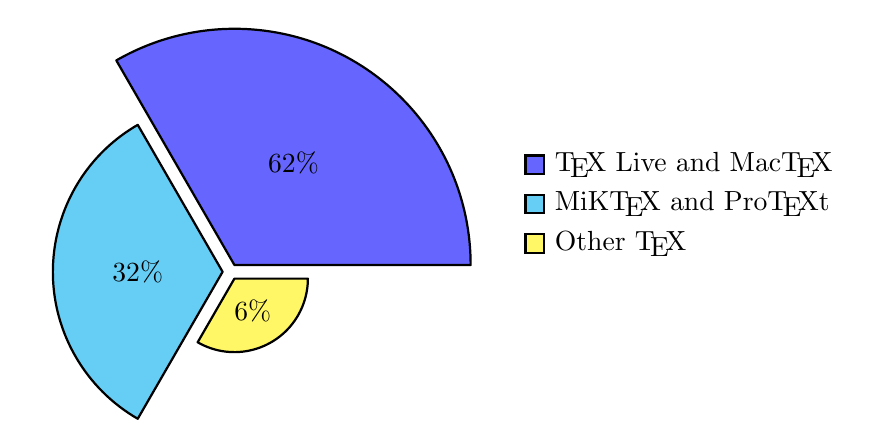
\begin{tikzpicture}
  \pie [polar, explode=0.1, text=legend]
    { 62/\TeX\ Live and Mac\TeX,
      32/MiK\TeX\ and Pro\TeX t, 6/Other \TeX }
\end{tikzpicture}
\end{document}

